% nofirafonts: the theme's default Fira Sans/Math fonts need firamath-otf,
% which requires XeLaTeX or LuaLaTeX. This deck targets pdflatex, so it
% opts out and falls back to Computer Modern via the documented class option.
\documentclass[10pt]{beamer}
\usetheme[nofirafonts]{focus}

\usepackage[utf8]{inputenc}
\usepackage[T1]{fontenc}
\usepackage{booktabs}
\usepackage{amsmath}
\usepackage{amssymb}
\usepackage{tikz}
\usetikzlibrary{arrows.meta,positioning,calc,fit}

% --------------------------------------------------------------------------
% Title block. The theme sets the title at display size; on a two-line title
% with a subtitle that runs under the author line, so the whole block is
% stepped down one size here.
% --------------------------------------------------------------------------
\setbeamerfont{title}{size=\large}
\setbeamerfont{subtitle}{size=\footnotesize}
\setbeamerfont{author}{size=\small}
\setbeamerfont{institute}{size=\footnotesize}
\setbeamerfont{date}{size=\footnotesize}

% --------------------------------------------------------------------------
% Artefact probing. The deck builds from report/ or from the repository root,
% so the path to the figures differs. Probe once against a figure the study
% always produces; fall back to labelled placeholders otherwise, so a partial
% run still yields a complete deck.
% --------------------------------------------------------------------------
\newcommand{\figroot}{}
\IfFileExists{../artifacts/figures/F1_feasibility.png}
  {\renewcommand{\figroot}{../artifacts/figures/}}{}
\IfFileExists{artifacts/figures/F1_feasibility.png}
  {\renewcommand{\figroot}{artifacts/figures/}}{}

% \plot{file}{what the reader should look for}
\newcommand{\plot}[2]{%
  \begin{center}%
  \IfFileExists{\figroot#1}%
    {\includegraphics[width=\linewidth,height=0.58\textheight,keepaspectratio]{\figroot#1}}%
    {\setlength{\fboxsep}{6pt}%
     \fbox{\parbox[c][0.50\textheight][c]{0.86\linewidth}{\centering\footnotesize
       \textbf{figure placeholder}\\[4pt]
       \texttt{\detokenize{#1}}\\[6pt]#2}}}%
  \end{center}}

% A cell awaiting the full-scale campaign, matching the report's convention.
\newcommand{\BL}{\textcolor{black!35}{\rule[0.35ex]{1.1em}{0.6pt}}}

% A one-line takeaway, always its own paragraph and always flushed to the
% foot of the frame, so it reads as a conclusion rather than as a continuation
% of whatever precedes it.
\newcommand{\takeaway}[1]{\par\vfill{\footnotesize\textbf{Reading.} #1\par}}

% Schematic styles, defined once.
\tikzset{
  blk/.style={draw, rounded corners=1.6pt, align=center, inner sep=3pt,
              font=\scriptsize, minimum height=6.5mm},
  fill1/.style={fill=black!6},
  fill2/.style={fill=black!14},
  sig/.style={-{Stealth[length=4pt,width=3pt]}, semithick},
  lbl/.style={font=\scriptsize, inner sep=1.5pt},
}

\title{Learning the Cost of a Wrong Model}
\subtitle{Adaptive actor--critic MPC with residual dynamics estimation
  for a quadrotor}
\author{BOUZID Amine}
\institute{Final-year project (PFE)}
\date{\today}

\begin{document}

\begin{frame}
  \titlepage
\end{frame}

\begin{frame}{Overview}
  \small
  \tableofcontents
\end{frame}

% ==========================================================================
\section{Context and objective}
% ==========================================================================

\begin{frame}{The operational problem}
  \begin{itemize}
    \item A quadrotor must track an aggressive reference under disturbances
      it was not designed for: wind, an off-centre payload, a mis-calibrated
      actuator.
    \item Model predictive control handles constraints and preview well, but
      its performance is bounded by the model it predicts with.
    \item On a real airframe the mismatch is not noise. It is structured,
      persistent, and specific to the vehicle.
  \end{itemize}
  \takeaway{The question is not how to remove model error, but what to do
    once it is accepted as permanent.}
\end{frame}

\begin{frame}{The scientific premise}
  \begin{block}{Gros and Zanon (2020)}
    For a \emph{wrong} model, the finite-horizon problem solved under that
    model still returns the optimal policy of the true system, provided its
    stage and terminal costs are adapted.
  \end{block}
  \vspace{4pt}
  Formally, for a true system $f^{\star}$ and a model $\hat f\neq f^{\star}$,
  there exist $\ell_\theta,\ V^f_\theta$ such that
  \[
    \pi_\theta(x)=\arg\min_{u_{0:N-1}}
      \sum_{k=0}^{N-1}\ell_\theta(x_k,u_k)+V^f_\theta(x_N)
    \quad\text{is optimal for } f^{\star}.
  \]
  \takeaway{The adapted cost is not computable in closed form, so it is
    \emph{learned} --- while the optimiser and its constraint handling are
    kept.}
\end{frame}

\begin{frame}{Where the learning sits}
  \centering
  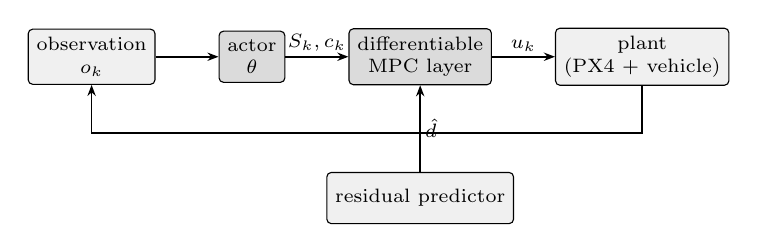
\begin{tikzpicture}[node distance=5mm]
    \node[blk,fill1] (obs) {observation\\$o_k$};
    \node[blk,fill2,right=8mm of obs] (actor) {actor\\$\theta$};
    \node[blk,fill2,right=8mm of actor] (mpc) {differentiable\\MPC layer};
    \node[blk,fill1,right=8mm of mpc] (plant) {plant\\(PX4 + vehicle)};
    \draw[sig] (obs) -- (actor);
    \draw[sig] (actor) -- node[lbl,above]{$S_k,c_k$} (mpc);
    \draw[sig] (mpc) -- node[lbl,above]{$u_k$} (plant);
    \draw[sig] (plant.south) -- ++(0,-6mm) -| (obs.south);
    \node[blk,fill1,below=11mm of mpc] (rdp) {residual predictor};
    \draw[sig] (rdp) -- node[lbl,right]{$\hat d$} (mpc);
  \end{tikzpicture}
  \takeaway{The policy gradient flows \emph{through} the solver. The
    constraint handling is never bypassed, only re-weighted.}
\end{frame}

\begin{frame}{Objectives and contributions}
  \begin{enumerate}
    \item A differentiable MPC layer whose stage cost is produced by a neural
      actor and trained by policy gradient.
    \item A causal residual dynamics predictor estimating the disturbance
      online and writing it into the prediction model.
    \item An incremental study: each addition measured against the one before
      it, on one protocol.
    \item A PX4/Gazebo workspace flying the result, sharing one
      implementation of the model with the study.
  \end{enumerate}
\end{frame}

% ==========================================================================
\section{Modelling}
% ==========================================================================

\begin{frame}{Conventions}
  \begin{itemize}
    \item World frame ENU, body frame FLU.
    \item Quaternion $q$ Hamilton, scalar first, body to world;
      $z_b(q)=R(q)e_3$.
    \item Control period $\Delta t_c=20\,$ms; the plant integrates at
      $\Delta t_c/10$.
    \item Two parameter sets throughout: the \emph{true} ones, which drive
      the plant, and the \emph{nominal} ones, which the controller and the
      autopilot's allocator believe.
  \end{itemize}
  \takeaway{Keeping both sets distinct is what makes model error exist by
    construction rather than by injection.}
\end{frame}

\begin{frame}{The actuator map}
  PX4 holds the rotors at an idle speed, so the normalised command maps
  \emph{affinely} to rotor speed and only then quadratically to thrust:
  {\small
  \[
    \Omega(c)=\Omega_{\min}+c\,(\Omega_{\max}-\Omega_{\min}),
    \quad
    T(c)=T_{\max}\big(r+c\,(1-r)\big)^{2},
    \quad r=\frac{\Omega_{\min}}{\Omega_{\max}} .
  \]}
  The hover collective gain follows by differentiation:
  {\small
  \[
    \left.\frac{\partial a_z}{\partial c}\right|_{\mathrm{hover}}
    =\frac{2T_{\max}(1-r)\big(r+u_{\mathrm{hover}}(1-r)\big)}{m}.
  \]}
  \takeaway{Setting $r=0$ --- the textbook $T=T_{\max}c^{2}$ --- misplaces
    hover, overstates control authority, and asserts the vehicle can produce
    zero thrust. All three mis-scale the terminal cost.}
\end{frame}

\begin{frame}{Allocation}
  {\small
  \[
    M=\begin{bmatrix}\mathbf 1^{\!\top}\\ M_\tau\end{bmatrix},
    \quad
    M_\tau=\begin{bmatrix}
      a_{1,y} & a_{2,y} & a_{3,y} & a_{4,y}\\
      -a_{1,x} & -a_{2,x} & -a_{3,x} & -a_{4,x}\\
      -\sigma_1k_m & -\sigma_2k_m & -\sigma_3k_m & -\sigma_4k_m
    \end{bmatrix},
    \quad a_i=r_i-\mathrm{cg}.
  \]}
  \begin{itemize}
    \item The \emph{allocator} inverts $M$ with the moment constant PX4
      carries in its airframe file.
    \item The \emph{plant} generates yaw moments from the simulator's rotor
      drag coefficient, which implies a far smaller effective arm.
  \end{itemize}
  \takeaway{The controller believes it has roughly three times the yaw
    authority it has. This is not an error to remove: it reproduces a
    disagreement present on the real stack.}
\end{frame}

\begin{frame}{Plant model, $23$ states}
  \[
    s=[\,\underbrace{p}_{3},\ \underbrace{q}_{4},\ \underbrace{v}_{3},\
        \underbrace{\omega}_{3},\ \underbrace{\Omega}_{4},\
        \underbrace{I_\omega}_{3},\ \underbrace{\omega_f}_{3}\,]\in\mathbb{R}^{23}
  \]
  \small
  \begin{align*}
    \dot v &= \frac{\sum_iK_T\Omega_i^{2}}{m}z_b-g\,e_3
      -\frac{D\odot(v-v_w)}{m}
      -\frac{c_{\mathrm{rd}}\sum_i\Omega_i\,v_\perp}{m}
      +\frac{R\,F^{b}_{\mathrm{ext}}}{m}\\
    \dot\omega &= J^{-1}\big(M_\tau K_T\Omega^{2}+\tau_{\mathrm{roll}}
      +\tau_{\mathrm{ext}}-\omega\times J\omega\big)\\
    \dot\Omega &= (\Omega_{\mathrm{cmd}}-\Omega)/\tau_m,\qquad
    \dot\omega_f = 2\pi f_{\mathrm{gyro}}(\omega-\omega_f),\qquad
    \dot I_\omega = \omega_c-\omega_f
  \end{align*}
  \normalsize
  \takeaway{Bulk drag, rotor drag and the rolling moment are the simulator's
    own aerodynamics. None of them appears in the control model.}
\end{frame}

\begin{frame}{The autopilot's rate loop}
  \begin{align*}
    \tau_{\mathrm{cmd}} &= J\big(K_r(\omega_c-\omega_f)+K_iI_\omega
      -K_d\omega_f\big)+\omega\times J\omega,\\
    f_{\mathrm{cmd}} &= \operatorname{clip}\big(M_{\mathrm{ctrl}}^{-1}
      [\,T_c,\ \tau_{\mathrm{cmd}}\,]^{\!\top},\
      T_{\mathrm{idle}}/4,\ f_{\max}\big),\qquad
    \Omega_{\mathrm{cmd}}=\sqrt{f_{\mathrm{cmd}}/K_T}.
  \end{align*}
  \begin{itemize}
    \item A PID on body rate, closed inside the autopilot at a rate the
      offboard controller cannot see.
    \item Its integrator drives $\omega_f\to\omega_c$, so its steady-state
      rate gain is exactly $\operatorname{diag}(\omega_{\max})$.
  \end{itemize}
  \takeaway{This loop is the fastest dynamics between the command and the
    attitude. A controller that ignores it is predicting a vehicle it is not
    flying.}
\end{frame}

\begin{frame}{Payload and wind}
  \textbf{Payload} shifts the centre of gravity and the inertia:
  {\small
  \[
    m_t=m_{\mathrm{air}}+m_p,\quad
    \mathrm{cg}=\frac{m_{\mathrm{air}}\,\mathrm{cg}_0+m_p\,r_p}{m_t},\quad
    J=J_{\mathrm{air}}+\sum_j m_j\big(\|d_j\|^{2}I-d_jd_j^{\!\top}\big).
  \]}
  \textbf{Wind} is per episode and deterministic in $t$:
  \[
    v_w(t)=\bar w\Big[\big(1+0.35\sin(2\pi\cdot0.23\,t+\phi)\big)\hat d
      +0.35\sin(2\pi\cdot0.7\,t)\,\hat d^{\perp}\Big].
  \]
  \takeaway{The arms are rebuilt about the shifted CG, so an off-centre
    payload produces a standing moment the allocator does not know about.}
\end{frame}

\begin{frame}{Two models, by design}
  \centering
  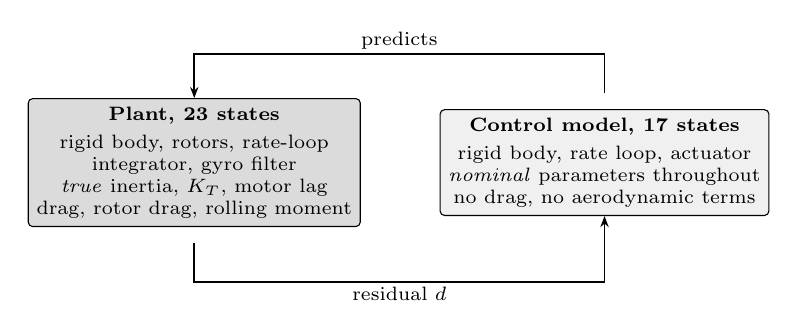
\begin{tikzpicture}[node distance=4mm]
    \node[blk,fill2,minimum width=34mm] (p) {\textbf{Plant, 23 states}\\[2pt]
      rigid body, rotors, rate-loop\\integrator, gyro filter\\
      \emph{true} inertia, $K_T$, motor lag\\ drag, rotor drag, rolling moment};
    \node[blk,fill1,minimum width=34mm,right=10mm of p] (c)
      {\textbf{Control model, 17 states}\\[2pt]
       rigid body, rate loop, actuator\\
       \emph{nominal} parameters throughout\\ no drag, no aerodynamic terms};
    \draw[sig] (c.north) ++(0,2mm) -- ++(0,5mm) -| node[lbl,pos=0.25,above]
      {predicts} (p.north);
    \draw[sig] (p.south) ++(0,-2mm) -- ++(0,-5mm) -| node[lbl,pos=0.25,below]
      {residual $d$} (c.south);
  \end{tikzpicture}
  \takeaway{The gap between the two boxes is the object of study. Using true
    parameters inside the optimiser would delete it.}
\end{frame}

\begin{frame}{Control model, $17$ states}
  \[
    x=[\,\underbrace{p}_{3},\ \underbrace{v}_{3},\ \underbrace{q}_{4},\
        \underbrace{\omega}_{3},\ \underbrace{\Omega}_{4}\,]\in\mathbb{R}^{17},
    \qquad
    u=[\,c,\ \bar\omega_x,\ \bar\omega_y,\ \bar\omega_z\,]\in\mathbb{R}^{4}
  \]
  \begin{itemize}
    \item The input is the CTBR command the autopilot actually exposes, so
      nothing about the deployment interface is assumed away.
    \item Carrying $\omega$ and $\Omega$ means the rate loop and the actuator
      are \emph{predicted}, not taken to be instantaneous.
    \item All constants nominal: a controller does not know the true inertia,
      rotor constant or motor lag.
  \end{itemize}
\end{frame}

\begin{frame}{Dynamics: inner loop and mixer}
  \small
  \begin{align*}
    \omega_c &= \operatorname{clip}\big(\operatorname{diag}(\omega_{\max})\,
      \bar\omega,\ \pm\omega_{\mathrm{lim}}\big)\\
    \tau_{\mathrm{cmd}} &= J_n\big(K_r\odot(\omega_c-\omega)\big)
      +\omega\times J_n\omega\\
    f_{\mathrm{cmd}} &= \operatorname{clip}\big(M_{\mathrm{ctrl}}^{-1}
      [\,T(c),\ \tau_{\mathrm{cmd}}\,]^{\!\top},\ 0,\ f_{\max}\big)\\
    \Omega_{\mathrm{cmd}} &= \operatorname{clip}\big(
      \sqrt{f_{\mathrm{cmd}}/K_T},\ \Omega_{\min},\ \Omega_{\max}\big)
  \end{align*}
  \normalsize
  \takeaway{A \emph{proportional} reduction of the autopilot's PID. The
    allocator and the idle-floor actuator map are reproduced exactly, with
    nominal constants.}
\end{frame}

\begin{frame}{Dynamics: rigid body and actuator}
  \small
  \begin{align*}
    \dot p &= v\\
    \dot v &= \frac{K_T\sum_i\Omega_i^{2}}{m}\,z_b(q)-g\,e_3+a_{\mathrm{res}}\\
    \dot q &= \tfrac12\,q\otimes[\,0,\ \omega\,]\\
    \dot\omega &= J_n^{-1}\big(M_\tau^{n}K_T\Omega^{2}
      -\omega\times J_n\omega\big)+\alpha_{\mathrm{res}}\\
    \dot\Omega &= (\Omega_{\mathrm{cmd}}-\Omega)/\tau_m
  \end{align*}
  \normalsize
  \takeaway{Integration is RK4 in two sub-steps over $\Delta t_c$: the rotor
    pole is \emph{faster} than the control period, so one step resolves the
    fastest mode only marginally.}
\end{frame}

\begin{frame}{The model is a cascade}
  \centering
  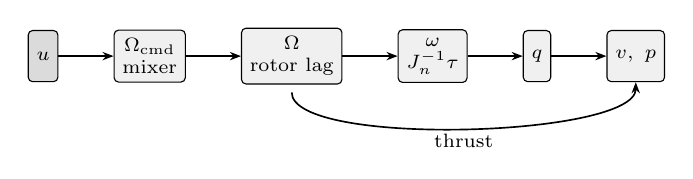
\begin{tikzpicture}[node distance=7mm]
    \node[blk,fill2] (u) {$u$};
    \node[blk,fill1,right=of u] (om) {$\Omega_{\mathrm{cmd}}$\\mixer};
    \node[blk,fill1,right=of om] (Om) {$\Omega$\\rotor lag};
    \node[blk,fill1,right=of Om] (w) {$\omega$\\$J_n^{-1}\tau$};
    \node[blk,fill1,right=of w] (q) {$q$};
    \node[blk,fill1,right=of q] (pv) {$v,\ p$};
    \draw[sig] (u)--(om); \draw[sig] (om)--(Om); \draw[sig] (Om)--(w);
    \draw[sig] (w)--(q); \draw[sig] (q)--(pv);
    \draw[sig] (Om.south) ++(0,-1mm) .. controls +(0,-7mm) and +(0,-7mm) ..
      node[lbl,below]{thrust} (pv.south);
  \end{tikzpicture}
  \vspace{4pt}
  \begin{block}{Consequence}
    $\partial\dot x/\partial u$ is supported on the rotor block alone, so the
    hover linearisation has $B_c=0$ on every row but that block.
  \end{block}
  \takeaway{The input reaches attitude only through two integrations. A model
    that lets $u$ act on attitude directly asserts an infinitely fast rate
    loop.}
\end{frame}

\begin{frame}{The steady-state gains are exact}
  \begin{block}{Proposition}
    Hold $u$ constant until $\dot\Omega=0$ and $\dot\omega=0$. Then
    \[
      \omega_\infty=\operatorname{diag}(\omega_{\max})\,\bar\omega,
      \qquad
      \left.\frac{\partial a_z}{\partial c}\right|_{\mathrm{hover}}
      =\frac{2T_{\max}(1-r)\big(r+u_{\mathrm{hover}}(1-r)\big)}{m}.
    \]
  \end{block}
  \emph{Proof sketch.} At $\dot\Omega=0$, $\Omega=\Omega_{\mathrm{cmd}}$, so
  the realised wrench equals the commanded one; substituting its moment part
  and setting $\dot\omega=0$ leaves $K_r\odot(\omega_c-\omega)=0$. For the
  collective, a symmetric change leaves the moment rows fixed, so
  $K_T\sum_i\Omega_i^{2}=T(c)$.
  \takeaway{This is why the inner loop drops $K_i$ and $K_d$ \emph{together}:
    keeping $K_d$ alone leaves a standing $2\%$ droop, which integrates into
    attitude rather than decaying.}
\end{frame}

\begin{frame}{Error coordinates}
  \[
    e=\begin{bmatrix}
      p-p_r\\ v-v_r\\ 2\operatorname{sgn}(q_{e,w})\,q_{e,v}\\
      \omega-\omega_r\\ (\Omega-\Omega_r)/\Omega_{\mathrm{sc}}
    \end{bmatrix}\in\mathbb{R}^{16},
    \qquad q_e=q_r^{*}\otimes q .
  \]
  \begin{itemize}
    \item The sign selects the shorter rotation; for a tilt $\vartheta$,
      $\|e_{7:9}\|=2\sin(\vartheta/2)$.
    \item The rate and rotor blocks are plain vector differences: neither
      lives on a manifold.
  \end{itemize}
  \takeaway{The reduction removes the quaternion's redundancy while staying a
    local diffeomorphism --- which the iLQR needs, since it linearises here.}
\end{frame}

\begin{frame}{Exact inverse of the attitude error}
  \begin{block}{Lemma}
    Let $\delta=2\operatorname{sgn}(q_{e,w})q_{e,v}$ with $\|\delta\|\le2$.
    The unique $q_e$ in the upper hemisphere is
    \[
      q_e=\big[\cos(n/2),\ \hat\delta\sin(n/2)\big],
      \qquad n=2\arcsin(\|\delta\|/2).
    \]
  \end{block}
  \emph{Implementation.} The algebraically identical closed form
  $q_e=[\sqrt{1-\|\delta\|^{2}/4},\ \delta/2]$ is used instead: the lemma's
  form divides by $\|\delta\|$, whose gradient is undefined at zero error ---
  exactly the point the solver linearises about at convergence.
  \takeaway{The shortcut $n\approx\|\delta\|$ is wrong by $2.7^\circ$ at
    $60^\circ$ and $20.8^\circ$ at $120^\circ$.}
\end{frame}

\begin{frame}{References by differential flatness}
  \begin{itemize}
    \item Position and its derivatives fix the attitude: $z_b\propto a_r+ge_3$
      determines $q_r$ up to yaw.
    \item $\omega_r$ from a centred difference of $q_r$;
      $\dot\omega_r$ from a centred difference of $\omega_r$.
    \item $\Omega_r$ from inverting the nominal allocator at the reference
      wrench:
      \[
        \tau_r=J_n\dot\omega_r+\omega_r\times J_n\omega_r,
        \qquad
        \Omega_r=\operatorname{clip}\Big(\sqrt{M_{\mathrm{ctrl}}^{-1}
          [\,T_r,\ \tau_r\,]^{\!\top}/K_T}\Big).
      \]
  \end{itemize}
  \takeaway{At hover $\tau_r=0$ and $T_r=mg$, so $\Omega_r$ is the trim speed
    and $e=0$ holds \emph{exactly} at trim --- a genuine equilibrium, not an
    approximate one.}
\end{frame}

\begin{frame}{Feasibility of the reference}
  \begin{itemize}
    \item The lateral acceleration budget is what remains once weight is
      carried:
      $a_{\mathrm{lat}}^{\max}=\sqrt{(T_{\max}/m)^{2}-g^{2}}$.
    \item Each family demands $a=R\omega^{2}\kappa_a$; the angular rate is
      capped so that $\alpha\,a_{\mathrm{lat}}^{\max}$ is never exceeded.
    \item Uncapped, the superellipse ``square'' demands several times the
      whole envelope at small radius.
  \end{itemize}
  \takeaway{A reference no controller can fly measures the reference, not the
    controller. Capping happens before any comparison.}
\end{frame}

% ==========================================================================
\section{The predictive control layer}
% ==========================================================================

\begin{frame}{Error dynamics along a moving reference}
  One stage, with $\delta u$ the increment on the flatness feed-forward:
  \[
    e_{k+1}=\operatorname{err}\!\big(
      \Phi(\,\iota(e_k,x_{r,k}),\ u_{r,k}+\delta u_k,\ d\,),\ x_{r,k+1}\big),
  \]
  where $\iota$ is the inverse of $\operatorname{err}$ and $\Phi$ one RK4 step
  of the control model.
  \begin{itemize}
    \item The reference advances \emph{within} the horizon.
    \item Freezing it is a bug, not a simplification: at $1.5\,$m/s over
      twenty stages the target travels $0.6\,$m.
  \end{itemize}
  \takeaway{Preview is what an online solve buys over a static feedback law.}
\end{frame}

\begin{frame}{The optimal control problem}
  With $N_\tau=N_e+N_u=20$ and $\tau_k=[\,e_k,\ \delta u_k\,]^{\!\top}$:
  \[
    \min_{\delta u_{0:N-1}}\
      \sum_{k=0}^{N-1}\Big(\tfrac12\tau_k^{\!\top}S_k\tau_k
        +c_k^{\!\top}\tau_k\Big)
      +\tfrac12 e_N^{\!\top}P_{\mathrm{term}}e_N
  \]
  \[
    \text{s.t.}\quad e_{k+1}=\text{(error dynamics)},
    \qquad \delta u_k\in[\,\underline u-u_r,\ \overline u-u_r\,].
  \]
  \begin{itemize}
    \item $S_k\succeq0$ and $c_k$ are what the actor produces.
    \item The box is the \emph{reachable} set: the autopilot clips the rate
      command well inside the nominal range.
  \end{itemize}
\end{frame}

\begin{frame}{Why constraints are relaxed, not enforced}
  \[
    h_\theta(x_k,u_k)\le\sigma_k,
    \qquad\text{penalty } w^{\!\top}\sigma_k,\quad \sigma_k\ge0 .
  \]
  \begin{itemize}
    \item Hard constraints make the value $+\infty$ on any violation.
    \item An infinite value carries no information in a temporal-difference
      update: the gradient is undefined exactly where learning is needed.
    \item The exact relaxation keeps the optimum unchanged when the
      constraint is satisfiable.
  \end{itemize}
  \takeaway{Any form of learning is meaningless if infinite penalties are
    assigned to violating limitations.}
\end{frame}

\begin{frame}{iLQR}
  \centering
  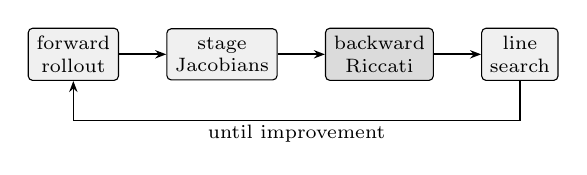
\begin{tikzpicture}[node distance=6mm]
    \node[blk,fill1] (r) {forward\\rollout};
    \node[blk,fill1,right=of r] (l) {stage\\Jacobians};
    \node[blk,fill2,right=of l] (b) {backward\\Riccati};
    \node[blk,fill1,right=of b] (s) {line\\search};
    \draw[sig] (r)--(l); \draw[sig] (l)--(b); \draw[sig] (b)--(s);
    \draw[sig] (s.south) -- ++(0,-5mm) -| node[lbl,below,pos=0.25]
      {until improvement} (r.south);
  \end{tikzpicture}
  \vspace{2pt}
  \small
  \begin{align*}
    Q_x &= \ell_x+A^{\!\top}V', &
    Q_{xx} &= \ell_{xx}+A^{\!\top}V''A,\\
    Q_u &= \ell_u+B^{\!\top}V', &
    Q_{uu} &= \ell_{uu}+B^{\!\top}V''B+\mu I,\\
    K &= -Q_{uu}^{-1}Q_{ux}, & k &= -Q_{uu}^{-1}Q_u .
  \end{align*}
  \normalsize
  \takeaway{$\mu$ is Levenberg--Marquardt regularisation: it is raised when a
    step fails and lowered when it succeeds.}
\end{frame}

\begin{frame}{Differentiating through the solve}
  \begin{itemize}
    \item The actor needs $\partial u^{\star}/\partial S_k$ and
      $\partial u^{\star}/\partial c_k$.
    \item Only the last few iterations carry gradient. At a solution
      satisfying second-order sufficiency, the parameter gradient depends on
      the optimum, not on the path taken to it.
    \item The clamp on the input box passes its derivative \emph{on} the
      boundary; choosing zero there would make $Q_{uu}$ singular exactly when
      the solver tries to come back inside.
  \end{itemize}
  \takeaway{This truncation costs accuracy only through the residual
    optimality gap, and buys a far smaller computational graph.}
\end{frame}

\begin{frame}{Increment 1: learned local terminal cost}
  \[
    P_\theta(e)=L_\theta(e)L_\theta(e)^{\!\top}+\varepsilon I\succ0,
    \qquad
    \min_\theta\ \mathbb{E}\big[(\tfrac12 e^{\!\top}P_\theta(e)e-V_1(e))^{2}\big]
  \]
  \begin{itemize}
    \item The terminal cost is the horizon's summary of everything beyond it;
      a Riccati matrix is only correct near the linearisation point.
    \item $V_1$ is the realised cost-to-go of a long solve from $e$.
    \item Positive definiteness is by construction, so the inner problem stays
      well posed.
  \end{itemize}
  \takeaway{The stage cost is left untouched, which isolates one question:
    how much does the terminal cost alone matter?}
\end{frame}

\begin{frame}{Increment 2: the learned cost map}
  {\small
  \[
    z=\mathrm{MLP}_\theta(o),
    \qquad
    c_k=P_{\mathrm{hi}}\tanh(z_p),
  \]
  \[
    S_k=\begin{cases}
      \operatorname{diag}\big(Q_{\mathrm{lo}}
        (Q_{\mathrm{hi}}/Q_{\mathrm{lo}})^{\sigma(z)}\big)
        & \text{diagonal}\\[2pt]
      A_kA_k^{\!\top}+Q_{\mathrm{lo}}I & \text{Cholesky, full}
    \end{cases}
  \]}
  \begin{itemize}
    \item Weights span five decades, so they are produced on a
      \emph{logarithmic} scale and bounded at both ends.
    \item $c_k$ is bounded symmetrically: in error coordinates the target is
      $e=0$, so a one-signed linear term would bias every channel.
    \item $P_{\mathrm{hi}}<\sqrt{Q_{\mathrm{lo}}Q_{\mathrm{hi}}}$, so the
      linear term shifts the optimum without dominating it.
  \end{itemize}
\end{frame}

% ==========================================================================
\section{Disturbance and adaptation}
% ==========================================================================

\begin{frame}{Two objects, one disturbance}
  \begin{columns}[T]
    \begin{column}{0.48\textwidth}
      \textbf{Model residual}
      \[
        d=\begin{bmatrix}
          a_{\mathrm{plant}}-a_{\mathrm{model}}\\
          \dot\omega_{\mathrm{plant}}-\dot\omega_{\mathrm{model}}
        \end{bmatrix}
      \]
      \footnotesize What the nominal model fails to explain, in the
      coordinates the model uses. Units m/s$^2$, rad/s$^2$.
    \end{column}
    \begin{column}{0.48\textwidth}
      \textbf{External wrench}
      \[
        w=\begin{bmatrix}F_{\mathrm{ext}}\\ \tau_{\mathrm{ext}}\end{bmatrix}
      \]
      \footnotesize What a force--torque sensor reads, and what the estimator
      is trained against. Units N, N$\,$m.
    \end{column}
  \end{columns}
  \takeaway{Confusing them is silent: it produces plausible numbers, wrong in
    the same direction every time, with no exception raised.}
\end{frame}

\begin{frame}{The conversion is exact}
  \begin{block}{Proposition}
    The two are related by an invertible, constant, block-diagonal map:
    \[
      d=\begin{bmatrix}m^{-1}I_3 & 0\\ 0 & J_n^{-1}\end{bmatrix}w,
      \qquad
      a_{\mathrm{res}}=\frac{F_{\mathrm{ext}}}{m},
      \qquad
      \alpha_{\mathrm{res}}=J_n^{-1}\tau_{\mathrm{ext}} .
    \]
  \end{block}
  \emph{Why it is structural.} The control model carries a torque input. A
  model whose deepest rotational state is attitude has no image for the moment
  block at all: a moment could only be represented through the rate offset it
  eventually produces, which depends on how long it has been acting.
  \takeaway{Measured against the plant, both blocks agree to a ratio of
    $1.000$ to machine precision.}
\end{frame}

\begin{frame}{What exactness does not buy}
  \begin{itemize}
    \item The nominal $m$ and $J_n$ in the conversion are \emph{not} the true
      ones --- by construction, and that difference is part of what the
      estimator must learn.
    \item The prediction stays approximate: the inner loop is a proportional
      reduction of a PID, so a moment the autopilot's integrator has absorbed
      is still predicted as a persistent angular acceleration.
  \end{itemize}
  \takeaway{The conversion removes an \emph{interface} error. It does not
    remove model error, which is the thing being learned.}
\end{frame}

\begin{frame}{The residual dynamics predictor}
  \centering
  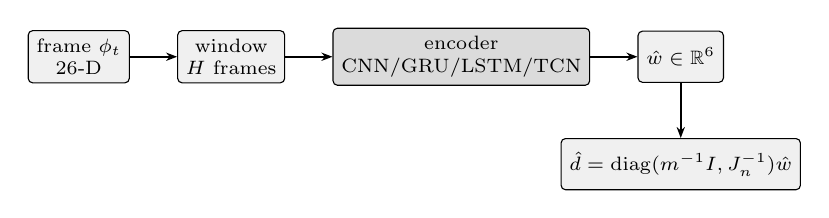
\begin{tikzpicture}[node distance=6mm]
    \node[blk,fill1] (fr) {frame $\phi_t$\\$26$-D};
    \node[blk,fill1,right=of fr] (win) {window\\$H$ frames};
    \node[blk,fill2,right=of win] (enc) {encoder\\CNN/GRU/LSTM/TCN};
    \node[blk,fill1,right=of enc] (out) {$\hat w\in\mathbb{R}^{6}$};
    \node[blk,fill1,below=7mm of out] (conv) {$\hat d=\mathrm{diag}(m^{-1}I,J_n^{-1})\hat w$};
    \draw[sig] (fr)--(win); \draw[sig] (win)--(enc); \draw[sig] (enc)--(out);
    \draw[sig] (out)--(conv);
  \end{tikzpicture}
  \vspace{2pt}
  \begin{itemize}
    \item Frame: $[\,p-p_r\ \|\ \mathrm{vec}(R)\ \|\ v\ \|\ \omega\ \|\
      u-u_r\ \|\ \mathrm{PWM}\,]$.
    \item \emph{Causal} by construction: no future sample enters the window.
  \end{itemize}
  \takeaway{Trained on position hold, where the disturbance response is not
    confounded with tracking.}
\end{frame}

\begin{frame}{Three ways to use the estimate}
  \begin{table}
    \centering
    \small
    \begin{tabular}{clp{0.48\linewidth}}
      \toprule
      Variant & Uses $\hat d$ as & Question it answers \\
      \midrule
      A & observation only & Does knowing the disturbance help the policy? \\
      B & model correction only & Does correcting the prediction help? \\
      C & both & Do the two compose? \\
      \bottomrule
    \end{tabular}
  \end{table}
  \takeaway{An oracle arm, fed the true disturbance, bounds what any
    estimator could deliver. The gap between oracle and estimator is what
    estimation quality costs.}
\end{frame}

% ==========================================================================
\section{Learning formulation}
% ==========================================================================

\begin{frame}{Markov decision process}
  {\footnotesize
  \[
    o=\big[\,\underbrace{e}_{16}\ \|\
      \underbrace{\{p_r(t{+}h\Delta)-p,\ v_r(t{+}h\Delta)\}_{h=1}^{3}}_{18}\ \|\
      \underbrace{\textstyle\int e_p}_{3}\ \|\
      \underbrace{\overline{\delta u}}_{4}\ \|\
      \underbrace{\overline{e_v}}_{3}\ \|\
      \underbrace{\overline{\omega}}_{3}\,\big]\in\mathbb{R}^{47}
  \]}
  \begin{itemize}
    \item Preview stride five control steps: lookaheads of $0.1/0.2/0.3\,$s.
    \item Running means are exponential, with a $0.5\,$s time constant.
    \item Normalised by a running mean and variance, the variance floored so
      near-constant channels are not amplified.
  \end{itemize}
  \takeaway{Disturbance-blind by default. The oracle and estimator channels
    are separate arms, added deliberately.}
\end{frame}

\begin{frame}{Reward}
  \[
    r=-\frac{e^{\!\top}Qe+\delta u^{\!\top}R\,\delta u}{100}
      -0.02\|\omega\|^{2}-0.05\|\Delta u\|^{2}
      -c_{\mathrm{crash}}\mathbb{1}_{\mathrm{crash}}
  \]
  \begin{itemize}
    \item The reward weights are a \emph{different object} from the MPC stage
      cost: one scores the closed loop, the other shapes an optimisation.
    \item Leaving the ball is priced as a failure. Otherwise the cheapest
      escape from a negative reward stream is to fly out of it.
    \item A shaped progress reward is available for the tracking curriculum.
  \end{itemize}
  \takeaway{Conflating reward and stage cost is a silent error: the cost
    weights are about $100\times$ too small to give the policy gradient any
    signal against the rate and increment penalties.}
\end{frame}

\begin{frame}{Policy optimisation}
  \[
    L(\theta)=\mathbb{E}\Big[\min\big(\rho_t\hat A_t,\
      \operatorname{clip}(\rho_t,1{-}\epsilon,1{+}\epsilon)\hat A_t\big)\Big],
    \qquad \rho_t=\frac{\pi_\theta(a_t|o_t)}{\pi_{\theta_{\mathrm{old}}}(a_t|o_t)}
  \]
  \[
    \hat A_t=\sum_{l\ge0}(\gamma\lambda)^{l}\delta_{t+l},
    \qquad \delta_t=r_t+\gamma V(o_{t+1})-V(o_t)
  \]
  \begin{itemize}
    \item The policy is Gaussian \emph{over the action}, not over the cost
      map: exploration must reach the quantity being studied.
    \item The step size is keyed to the measured KL --- the MPC mean is far
      more sensitive to its cost map than an MLP's output is to its weights.
  \end{itemize}
\end{frame}

% ==========================================================================
\section{Data and protocol}
% ==========================================================================

\begin{frame}{The data-generating process}
  \begin{itemize}
    \item There is no fixed dataset. Episodes are \emph{sampled}, and the
      sampler is part of the method.
    \item Per episode: reference family, radius, phase, speed, centre, initial
      offset, wind magnitude and direction.
    \item Per episode: multiplicative parameter factors
      $\lambda_m,\lambda_D,\lambda_\tau,\lambda_T,\lambda_{K_w},\lambda_J$.
    \item Termination on crash, on leaving a $3\,$m ball, on excessive spin,
      or on episode length; the vehicle is resampled in place.
  \end{itemize}
  \takeaway{Batched environments make the episode boundary an artefact, so
    truncation is bootstrapped rather than cut.}
\end{frame}

\begin{frame}{Randomisation suites}
  \begin{table}
    \centering
    \small
    \begin{tabular}{lccc}
      \toprule
      Axis & S1 nominal & S2 disturbed & S3 out of distribution \\
      \midrule
      speed [m/s]      & $0.5$--$1.5$ & $0.5$--$4.0$ & $5.0$--$6.5$ \\
      wind [m/s]       & $0$          & $0$--$15$    & $18$--$25$ \\
      mass $\lambda_m$ & $1$          & $0.80$--$1.20$ & $0.65$--$1.35$ \\
      drag $\lambda_D$ & $1$          & $0.50$--$2.00$ & $2.20$--$3.00$ \\
      motor $\lambda_\tau$ & $1$      & $0.50$--$3.00$ & $3.50$--$5.00$ \\
      inertia $\lambda_J$ & $1$       & $0.70$--$1.40$ & $0.50$--$1.80$ \\
      \bottomrule
    \end{tabular}
  \end{table}
  \takeaway{The raw suites saturate every controller, so they are moderated
    before evaluation --- and the moderation is reported, not hidden.}
\end{frame}

\begin{frame}{Training scales}
  \begin{table}
    \centering
    \small
    \begin{tabular}{lrrr}
      \toprule
      & smoke & medium & full \\
      \midrule
      parallel environments & $16$ & $128$ & $512$ \\
      rollout length        & $16$ & $32$  & $64$ \\
      iterations            & $6$  & $80$  & $400$ \\
      hidden width          & $64$ & $256$ & $1024$ \\
      iLQR iterations       & $5$  & $10$  & $25$ \\
      \bottomrule
    \end{tabular}
  \end{table}
  \takeaway{Only \emph{full} rows are results. Smaller scales produce
    undertrained policies by construction and exist to verify the pipeline,
    not to support a claim.}
\end{frame}

\begin{frame}{Metrics, and why each}
  \begin{table}
    \centering
    \small
    \begin{tabular}{lp{0.56\linewidth}}
      \toprule
      Metric & Why it is reported \\
      \midrule
      Position RMSE & The task, but alone it is a trap under disturbance \\
      Saturation fraction & Distinguishes controllers that all hit the bound \\
      Crash rate & A low RMSE over surviving episodes means nothing alone \\
      Tilt & Separates aggressive recovery from instability \\
      Solve latency & Measured on a batch of \emph{one}, against $20\,$ms \\
      \bottomrule
    \end{tabular}
  \end{table}
  \takeaway{Throughput divided by batch size is a different quantity and
    flatters the learned controllers by orders of magnitude.}
\end{frame}

\begin{frame}{Statistical treatment}
  \begin{itemize}
    \item Seeds are the unit of variation; a difference smaller than the seed
      spread is not a result.
    \item Spread reported as an interquartile range over vehicles, not a
      standard error over steps --- steps within an episode are not
      independent.
    \item The same evaluation environments, seeds and episode lengths across
      every controller class.
  \end{itemize}
  \takeaway{The seed spread is the scale against which every other difference
    in the study is judged.}
\end{frame}

\begin{frame}{The increment chain}
  \centering
  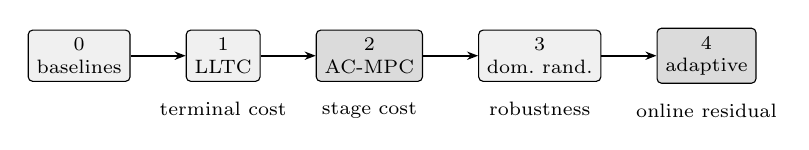
\begin{tikzpicture}[node distance=7mm]
    \node[blk,fill1] (i0) {0\\baselines};
    \node[blk,fill1,right=of i0] (i1) {1\\LLTC};
    \node[blk,fill2,right=of i1] (i2) {2\\AC-MPC};
    \node[blk,fill1,right=of i2] (i3) {3\\dom.\ rand.};
    \node[blk,fill2,right=of i3] (i4) {4\\adaptive};
    \draw[sig] (i0)--(i1); \draw[sig] (i1)--(i2);
    \draw[sig] (i2)--(i3); \draw[sig] (i3)--(i4);
    \node[lbl,below=2mm of i1] {terminal cost};
    \node[lbl,below=2mm of i2] {stage cost};
    \node[lbl,below=2mm of i3] {robustness};
    \node[lbl,below=2mm of i4] {online residual};
  \end{tikzpicture}
  \takeaway{Each increment must beat the one before it on the same protocol,
    or it does not earn its complexity.}
\end{frame}

% ==========================================================================
\section{Results}
% ==========================================================================

\begin{frame}{The reference must be flyable}
  \plot{F1_feasibility.png}{Demanded lateral acceleration per reference
    family, against the budget left once weight is carried.}
  \takeaway{The infeasible families are capped before any comparison, so the
    tables measure controllers rather than references.}
\end{frame}

\begin{frame}{What an online solve buys}
  \plot{F3_horizon.png}{Tracking error against horizon length, with and
    without reference preview, and the matching solve latency.}
  \takeaway{Preview is the mechanism, not horizon length as such: with the
    reference frozen, a longer horizon makes tracking \emph{worse}.}
\end{frame}

\begin{frame}{How much of the result is weight tuning}
  \plot{F5_qr_heatmap.png}{Closed-loop RMSE over the admissible
    $(Q_{\mathrm{pos}},R)$ grid.}
  \takeaway{The best-to-worst ratio over this grid is the fraction of
    ``controller performance'' that is really tuning effort --- and it is
    what a learned cost is meant to remove.}
\end{frame}

\begin{frame}{The learned terminal cost}
  \plot{F6_lltc_fit.png}{Fit quality of $P_\theta$ against the realised
    cost-to-go, in and out of the sampled shell.}
  \takeaway{A better fit to a worse controller is the signal that the fit
    \emph{target}, not the sampling, limits this arm.}
\end{frame}

\begin{frame}{Cost-map parametrisation}
  \plot{F9_representations.png}{Learning curves for the diagonal, Cholesky
    and full parametrisations.}
  \takeaway{The three do not start from comparable initialisations, which
    predicts that the richer forms need \emph{longer} --- not that they are
    incapable.}
\end{frame}

\begin{frame}{The learned cost is not a rescaling}
  \plot{F12_interpretability.png}{Learned diagonal stage weights against the
    hand-tuned ones, per channel, on a logarithmic scale.}
  \takeaway{The ratio spans orders of magnitude and is not uniform across
    channels, so the learned cost is a distinct object.}
\end{frame}

\begin{frame}{Robustness by randomisation}
  \plot{F13_axis_competence.png}{Tracking error against each randomised
    parameter axis, for policies trained nominally and with randomisation.}
  \takeaway{Randomisation buys robustness where the axis is actually
    exercised in training; elsewhere it costs nominal performance without
    return.}
\end{frame}

\begin{frame}{The residual predictor}
  \plot{F16_encoder_trade.png}{Prediction quality against $95$th-percentile
    inference latency, per encoder, marker size proportional to parameter
    count.}
  \takeaway{The deadline is $20\,$ms. An encoder that misses it is not a
    candidate, whatever its accuracy.}
\end{frame}

\begin{frame}{Per-channel estimation quality}
  \plot{F17_channel_r2.png}{Coefficient of determination per wrench channel,
    for the selected encoder.}
  \takeaway{Force channels are easier than moment channels: a moment is
    observable only through its effect on the rate loop.}
\end{frame}

\begin{frame}{Adaptive closed loop}
  \plot{F18_closed_loop.png}{Closed-loop performance across scenarios, for
    the blind, oracle and estimator arms.}
  \takeaway{The oracle bounds what any estimator could deliver; the gap to
    the estimator arm is what estimation quality still costs.}
\end{frame}

\begin{frame}{Headline: accuracy against latency}
  \plot{F21_headline.png}{Every controller class on one plane: accuracy
    against single-vehicle solve latency, marker size proportional to the
    number of hand-tuned parameters.}
  \takeaway{The comparison that matters is accuracy per millisecond and per
    hand-tuned parameter, not accuracy alone.}
\end{frame}

\begin{frame}{Summary ledger}
  \begin{table}
    \centering
    \small
    \begin{tabular}{lrrrrr}
      \toprule
      Controller & S1 & S2 & S3 & p95 [ms] & tuned \\
      \midrule
      LQR $+$ feed-forward   & 0.0945 & 0.1882 & 0.3079 & 0.42 & 13 \\
      NMPC $N{=}1$           & 0.0739 & 0.1275 & 0.2368 & 12.04 & 13 \\
      NMPC $N{=}10$          & 0.0699 & 0.0993 & 0.1986 & \alert{126.69} & 13 \\
      LLTC $N{=}1$           & 1.2547 & 1.2921 & 1.3202 & 12.20 & 13 \\
      AC-MPC $N{=}1$         & 0.1040 & 0.1657 & 0.2712 & 12.17 & \textbf{0} \\
      Adaptive AC-MPC $N{=}1$ & 0.1022 & 0.1561 & 0.2534 & 12.56 & \textbf{0} \\
      \bottomrule
    \end{tabular}
  \end{table}
  \takeaway{RMSE in metres; \texttt{medium} scale; seed spread $0.0064\,$m is
    the resolution. \alert{$N{=}10$ misses the $20\,$ms period} --- the only
    row that is inadmissible. The last column is the claim: thirteen
    hand-chosen constants go to zero, and S1 accuracy pays about $41\,\%$
    for it.}
\end{frame}

% ==========================================================================
\section{PX4, ROS 2 and Gazebo}
% ==========================================================================

\begin{frame}{Why a deployment half at all}
  \begin{itemize}
    \item A controller that exists only inside its own simulator has not been
      shown to be a controller.
    \item The workspace imports the \emph{study module} for the model and the
      solver rather than carrying a second implementation.
    \item A duplicated dynamics model would be a second thing to keep in step,
      with no test able to see the divergence.
  \end{itemize}
  \takeaway{One model, one solver, one set of constants --- asserted by a
    cross-check, not by convention.}
\end{frame}

\begin{frame}{Software-in-the-loop architecture}
  \centering
  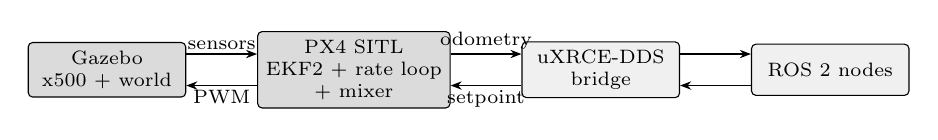
\begin{tikzpicture}[node distance=6mm]
    \node[blk,fill2,minimum width=20mm] (gz) {Gazebo\\x500 + world};
    \node[blk,fill2,minimum width=20mm,right=9mm of gz] (px4)
      {PX4 SITL\\EKF2 + rate loop\\+ mixer};
    \node[blk,fill1,minimum width=20mm,right=9mm of px4] (dds)
      {uXRCE-DDS\\bridge};
    \node[blk,fill1,minimum width=20mm,right=9mm of dds] (ros)
      {ROS 2 nodes};
    \draw[sig] ([yshift=2mm]gz.east) -- node[lbl,above]{sensors}
      ([yshift=2mm]px4.west);
    \draw[sig] ([yshift=-2mm]px4.west) -- node[lbl,below]{PWM}
      ([yshift=-2mm]gz.east);
    \draw[sig] ([yshift=2mm]px4.east) -- node[lbl,above]{odometry}
      ([yshift=2mm]dds.west);
    \draw[sig] ([yshift=-2mm]dds.west) -- node[lbl,below]{setpoint}
      ([yshift=-2mm]px4.east);
    \draw[sig] ([yshift=2mm]dds.east) -- ([yshift=2mm]ros.west);
    \draw[sig] ([yshift=-2mm]ros.west) -- ([yshift=-2mm]dds.east);
  \end{tikzpicture}
  \takeaway{The autopilot is \emph{inside} the loop. Its rate controller and
    mixer are the ones the $17$-state model reproduces.}
\end{frame}

\begin{frame}{The ROS 2 node graph}
  \centering
  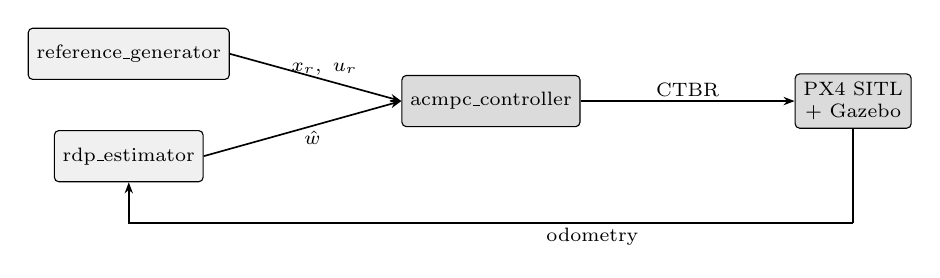
\begin{tikzpicture}[x=1mm,y=1mm]
    \node[blk,fill1] (ref) at (0,9)   {reference\_generator};
    \node[blk,fill1] (est) at (0,-4)  {rdp\_estimator};
    \node[blk,fill2] (ctl) at (46,3)  {acmpc\_controller};
    \node[blk,fill2] (px4) at (92,3)  {PX4 SITL\\+ Gazebo};
    \draw[sig] (ref.east) -- node[lbl,above,pos=0.55]{$x_r,\ u_r$} (ctl.west);
    \draw[sig] (est.east) -- node[lbl,below,pos=0.55]{$\hat w$} (ctl.west);
    \draw[sig] (ctl.east) -- node[lbl,above]{CTBR} (px4.west);
    \draw[semithick] (px4.south) -- ($(px4.south)+(0,-12)$);
    \draw[sig] ($(px4.south)+(0,-12)$) -|
      node[lbl,below,pos=0.18]{odometry} (est.south);
  \end{tikzpicture}
  \vspace{3pt}
  \begin{itemize}
    \footnotesize
    \item \texttt{state\_logger} records ground truth for offline evaluation.
    \item \texttt{disturbance\_manager} applies the scripted wrench in
      simulation; both also subscribe to the odometry bus.
  \end{itemize}
  \takeaway{The estimator is deliberately framework-free NumPy, so the flight
    path does not depend on the training stack.}
\end{frame}

\begin{frame}{Frames and the command interface}
  \begin{columns}[T]
    \begin{column}{0.46\textwidth}
      \small
      \textbf{PX4} publishes NED / FRD.\\[2pt]
      \textbf{Study} works in ENU / FLU.
      \[
        p_{\mathrm{ENU}}=\begin{bmatrix}0&1&0\\1&0&0\\0&0&-1\end{bmatrix}
        p_{\mathrm{NED}}
      \]
    \end{column}
    \begin{column}{0.50\textwidth}
      \small
      \textbf{Published each step}
      \begin{itemize}
        \footnotesize
        \item \texttt{OffboardControlMode} with body rate true
        \item \texttt{VehicleRatesSetpoint}: roll, pitch, yaw rates and a
          normalised, down-positive thrust
      \end{itemize}
    \end{column}
  \end{columns}
  \takeaway{Conversion happens \emph{on entry}, once, in one place. Frame
    errors are silent and systematic, so they are handled by construction
    rather than by inspection.}
\end{frame}

\begin{frame}{The rotor-speed observer}
  \begin{itemize}
    \item PX4 publishes no rotor speed, yet the control model carries
      $\Omega$ as a state.
    \item The controller propagates its own estimate from the commands it has
      sent, through the same integrator the prediction uses:
      $\hat\Omega_{k+1}=\Phi_\Omega(\hat\Omega_k,u_k)$.
    \item The mode is stable and fast, so the estimate converges from a cold
      start within a few control periods.
  \end{itemize}
  \takeaway{A coarse $\Omega$ is worth more than none: even at cold-start
    error the prediction improves on a model that omits the actuator.}
\end{frame}

\begin{frame}{Numerical parity}
  \begin{itemize}
    \item The wrench-to-residual conversion is implemented \emph{once} for
      the workspace and asserted against the study's on random wrenches.
    \item The $17$-state reference builder is checked against the study's
      across sampled times, in both the state and the feed-forward command.
    \item The exported estimator is replayed and compared with the trained
      one before it is written to disk.
  \end{itemize}
  \takeaway{Every constant that appears twice is asserted equal at import.
    A silent divergence between study and workspace is the failure mode these
    checks exist to prevent.}
\end{frame}

\begin{frame}{Latency budget}
  \begin{table}
    \centering
    \small
    \begin{tabular}{lrr}
      \toprule
      Stage & Median [ms] & p95 [ms] \\
      \midrule
      Residual estimation (GRU) & 1.23 & 1.24 \\
      MPC solve, $N{=}1$        & 12.40 & 12.56 \\
      \midrule
      Total, against $20\,$ms   & \textbf{13.63} & \textbf{13.80} \\
      \bottomrule
    \end{tabular}
  \end{table}
  \takeaway{$69\,\%$ of the period at p95, with $6.2\,$ms of margin. The first
    solve pays compilation; the budget is measured after warm-up, on a batch of
    one, which is the only quantity comparable to the control period. Batched
    throughput is a different number and is not this one.}
\end{frame}

\begin{frame}{Simulated scenarios}
  \plot{gazebo_scenarios.png}{Screenshots of the PX4/Gazebo x500 under the
    scripted scenarios: nominal, wind, centred payload, off-centre payload.}
  \takeaway{The scenarios mirror the randomisation axes used in training, so
    the simulated flight tests the failure modes the study measured.}
\end{frame}

\begin{frame}{Flight results}
  \plot{gazebo_tracking.png}{Commanded and realised trajectory, with the
    estimated wrench overlaid on the applied one.}
  \takeaway{The comparison to make is estimate against applied disturbance,
    not tracking error alone: a good tracker with a bad estimate has learned
    to reject, not to predict.}
\end{frame}

\begin{frame}{What is flown, and what is not}
  \begin{columns}[T]
    \begin{column}{0.48\textwidth}
      \textbf{Flown}
      \begin{itemize}
        \footnotesize
        \item PX4 software-in-the-loop with Gazebo
        \item The full node graph at the control rate
        \item Scripted disturbance scenarios
      \end{itemize}
    \end{column}
    \begin{column}{0.48\textwidth}
      \textbf{Not flown}
      \begin{itemize}
        \footnotesize
        \item Hardware in the loop
        \item A physical airframe
        \item Outdoor conditions
      \end{itemize}
    \end{column}
  \end{columns}
  \takeaway{Stating the boundary is part of the result. SITL validates the
    interfaces, the frames and the budget --- not the aerodynamics.}
\end{frame}

% ==========================================================================
\section{Conclusion}
% ==========================================================================

\begin{frame}{What the study establishes}
  \begin{itemize}
    \item A cost learned inside the optimiser is a distinct object from a
      tuned one, and the tuning spread it removes is measurable.
    \item Carrying the rate loop and the actuator in the prediction model
      makes the disturbance interface exact in both blocks.
    \item Each increment is reported against the one before it, on one
      protocol, with saturation beside accuracy.
    \item One model and one solver are shared by the study and the flight
      workspace, and the sharing is asserted rather than assumed.
  \end{itemize}
\end{frame}

\begin{frame}{Limitations}
  \begin{itemize}
    \item The rate loop is reduced, not reproduced: a long-standing moment is
      still predicted as a persistent angular acceleration.
    \item The cost parametrisation must stay quasi-convex for the inner solve
      to remain tractable, which bounds its richness.
    \item Seed counts are small relative to some of the differences claimed.
    \item Validation is software-in-the-loop only.
  \end{itemize}
\end{frame}

\begin{frame}{Future work}
  \begin{itemize}
    \item Restore the rate-loop integrator and measure whether it earns its
      three states.
    \item Sum-of-squares cost parametrisations: richer than a quadratic while
      still tractable.
    \item A GPU-resident solver, so horizon length stops trading against
      control rate.
    \item Hardware in the loop, then a physical airframe.
  \end{itemize}
\end{frame}

\begin{frame}
  \centering
  \Large Thank you
\end{frame}

\end{document}
